% ------------------------------------------------------------------------
% ------------------------------------------------------------------------
% Modelo para Trabalhos Acadêmicos (tese de doutorado, dissertação de mestrado) utilizando a classe abntex2
%
% 	Modificações:
%	- 31/03/2022: Henrique V. Lima, adequação do template para a Unievangélica
% ------------------------------------------------------------------------
% ------------------------------------------------------------------------

\documentclass[
	% -- opções da classe memoir --
	12pt,				% tamanho da fonte
	%openright,			% capítulos começam em pág ímpar (insere página vazia caso preciso)
	oneside,			% para impressão no anverso. Oposto a twoside
	a4paper,			% tamanho do papel. 
	% -- opções da classe abntex2 --
	chapter=TITLE,		% títulos de capítulos convertidos em letras maiúsculas
	section=TITLE,		% títulos de seções convertidos em letras maiúsculas
	%subsection=TITLE,	% títulos de subseções convertidos em letras maiúsculas
	%subsubsection=TITLE,% títulos de subsubseções convertidos em letras maiúsculas
	% -- opções do pacote babel --
	english,			% idioma adicional para hifenização
	%french,				% idioma adicional para hifenização
	%spanish,			% idioma adicional para hifenização
	brazil				% o último idioma é o principal do documento
	]{abntex2}

\usepackage{setup/ufscthesisA4-alf}
\usepackage{multirow}
\usepackage[table,xcdraw]{xcolor}
\usepackage{graphicx}
\usepackage{enumitem}
\usepackage[utf8]{inputenc}
% \usepackage[T1]{fontenc}
% \usepackage{lmodern}
% \usepackage{microtype}
% \usepackage[spanish]{babel}
% \usepackage{float}
% \usepackage{caption}
% \usepackage{booktabs}
% \usepackage{blindtext}
% \usepackage{siunitx}
% \usepackage{amssymb}

% ---
% Filtering and Mapping Bibliographies
% ---
% Pacotes de citações
% ---
\usepackage{csquotes}
\usepackage[backend = biber, style = abnt]{biblatex}
% FIXME Se desejar estilo numérico de citações,  comente a linha acima e descomente a linha a seguir.
% \usepackage[backend = biber, style = numeric-comp]{biblatex}

\setlength\bibitemsep{\baselineskip}
\DeclareFieldFormat{url}{Disponível~em:\addspace\url{#1}}
\NewBibliographyString{sineloco}
\NewBibliographyString{sinenomine}
\DefineBibliographyStrings{brazil}{%
	sineloco     = {\mkbibemph{S\adddot l\adddot}},
	sinenomine   = {\mkbibemph{s\adddot n\adddot}},
	andothers    = {\mkbibemph{et\addabbrvspace al\adddot}},
	in			 = {\mkbibemph{In:}}
}

\addbibresource{aftertext/references.bib} % Seus arquivos de referências

% ---
\DeclareSourcemap{
	\maps[datatype=bibtex]{
		% remove fields that are always useless
		\map{
			\step[fieldset=abstract, null]
			\step[fieldset=pagetotal, null]
		}
		% remove URLs for types that are primarily printed
%		\map{
%			\pernottype{software}
%			\pernottype{online}
%			\pernottype{report}
%			\pernottype{techreport}
%			\pernottype{standard}
%			\pernottype{manual}
%			\pernottype{misc}
%			\step[fieldset=url, null]
%			\step[fieldset=urldate, null]
%		}
		\map{
			\pertype{inproceedings}
			% remove mostly redundant conference information
			\step[fieldset=venue, null]
			\step[fieldset=eventdate, null]
			\step[fieldset=eventtitle, null]
			% do not show ISBN for proceedings
			\step[fieldset=isbn, null]
			% Citavi bug
			\step[fieldset=volume, null]
		}
	}
}
% ---

% ---
% Informações de dados para CAPA e FOLHA DE ROSTO
% ---
% FIXME Substituir 'Nome completo do autor' pelo seu nome.
\autor{Caio Alexandre Reis de Almeida \\ Lucas Gabriel de Brito Monteiro \\ Marcus Paulo Ribeiro Rodrigues Alves \\ Thiago Henrique Bueno de Oliveira}
% FIXME Substituir 'Título do trabalho' pelo título da trabalho.
\titulo{Empregai}
% FIXME Substituir 'Subtítulo (se houver)' pelo subtítulo da trabalho.  
% Caso não tenha substítulo, comente a linha a seguir.
\subtitulo{Sistema facilitador para contratação de serviços gerais}
% FIXME Substituir 'XXXXXX' pelo nome do seu
% orientador. WILLIAM PEREIRA DOS SANTOS JUNIOR
\orientador{Prof. William Pereira dos Santos Junior, Me.}
% FIXME Se for orientado por uma mulher, comente a linha acima e descomente a linha a seguir.
% \orientador[Orientadora]{Nome da orientadora, Dra.}
% FIXME Substituir 'XXXXXX' pelo nome do seu
% coorientador. Caso não tenha coorientador, comente a linha a seguir.
% \coorientador{Prof. XXXXXX, Dr.}
% FIXME Se for coorientado por uma mulher, comente a linha acima e descomente a linha a seguir.
% \coorientador[Coorientadora]{XXXXXX, Dra.}
% FIXME Substituir 'XXXXXX' pelo nome do Coordenador do 
% programa/curso.
% \coordenador{Prof. Natasha Sophie Pereira, Me.}
% FIXME Se for coordenadora mulher, comente a linha acima e descomente a linha a seguir.
\coordenador[Coordenadora]{Prof. Natasha Sophie Pereira, Me.}
% FIXME Substituir '[ano da entrega]' pelo ano (ano) em que seu trabalho foi defendido.
\ano{2023}
% FIXME Substituir '[dia] de [mês] de [ano]' pela data em que ocorreu sua defesa.
\data{[dia] de [mês] de [ano]}
% FIXME Substituir '[Cidade da defesa]' pela cidade em que ocorreu sua defesa.
\local{Anápolis}
\instituicaosigla{UNIEVANGÉLICA}
\instituicao{Universidade Evangélica de Goiás}
% FIXME Substituir 'Dissertação/Tese' pelo tipo de trabalho (Tese, Dissertação). 
\tipotrabalho{Trabalho de Conclusão de Curso}
% FIXME Substituir '[licenciado/bacharel] em [nome do título obtido]' pela grau adequado.
\formacao{bacharel em Engenharia de Software}
% FIXME Substituir '[licenciado/bacharel]' pelo nivel adequado.
\nivel{bacharel}
% FIXME Substituir 'Curso de Graduação em [XXXXXXXX]' pela curso adequado.
\programa{Curso de Graduação em Engenharia de Software}
% FIXME Substituir 'Campus XXXXXX ou Centro de XXXXXX' pelo campus ou centro adequado.
%\centro{Campus [XXXXXX] ou Centro de [XXXXXX]}
\preambulo
{%
\imprimirtipotrabalho~do~\imprimirprograma~do~\imprimircentro~da~\imprimirinstituicao~para~a~obtenção~do~título~de~\imprimirformacao.
}
% ---

% ---
% Configurações de aparência do PDF final
% ---
% alterando o aspecto da cor azul
\definecolor{blue}{RGB}{41,5,195}
% informações do PDF
\makeatletter
\hypersetup{
     	%pagebackref=true,
		pdftitle={\@title}, 
		pdfauthor={\@author},
    	pdfsubject={\imprimirpreambulo},
	    pdfcreator={LaTeX with abnTeX2},
		pdfkeywords={ufsc, latex, abntex2}, 
		colorlinks=true,       		% false: boxed links; true: colored links
    	linkcolor=black,%blue,          	% color of internal links
    	citecolor=black,%blue,        		% color of links to bibliography
    	filecolor=black,%magenta,      		% color of file links
		urlcolor=black,%blue,
		bookmarksdepth=4
}
\makeatother
% ---

% ---
% compila a lista de abreviaturas e siglas e a lista de símbolos
% ---

% Declaração das siglas
\siglalista{ABNT}{Associação Brasileira de Normas Técnicas}

% Declaração dos simbolos
\simbololista{C}{\ensuremath{C}}{Circunferência de um círculo}
\simbololista{pi}{\ensuremath{\pi}}{Número pi} 
\simbololista{r}{\ensuremath{r}}{Raio de um círculo}
\simbololista{A}{\ensuremath{A}}{Área de um círculo}

% compila a lista de abreviaturas e siglas e a lista de símbolos
\makenoidxglossaries 

% ---

% ---
% compila o indice
% ---
\makeindex
% ---

% ----
% Início do documento
% ----
\begin{document}

% Seleciona o idioma do documento (conforme pacotes do babel)
%\selectlanguage{english}
\selectlanguage{brazil}

% Retira espaço extra obsoleto entre as frases.
\frenchspacing 

% Espaçamento 1.5 entre linhas
\OnehalfSpacing

% Corrige justificação
%\sloppy

% ----------------------------------------------------------
% ELEMENTOS PRÉ-TEXTUAIS
% ----------------------------------------------------------
% \pretextual %a macro \pretextual é acionado automaticamente no início de \begin{document}
% ---
% Capa, folha de rosto, ficha bibliografica, errata, folha de apróvação
% Dedicatória, agradecimentos, epígrafe, resumos, listas
% ---
% ---
% Capa
% ---
\imprimircapa
% ---

% ---
% Folha de rosto
% (o * indica que haverá a ficha bibliográfica)
% ---
% \imprimirfolhaderosto*
% ---


% ---
% Inserir folha de aprovação
% ---
\begin{folhadeaprovacao}
	\OnehalfSpacing
	\centering
	\imprimirautor\\%
	\vspace*{10pt}		
	\textbf{\imprimirtitulo}%
	\ifnotempty{\imprimirsubtitulo}{:~\imprimirsubtitulo}\\%
	%		\vspace*{31.5pt}%3\baselineskip
	\vspace*{\baselineskip}
	%\begin{minipage}{\textwidth}
	% ~do~\imprimirprograma~do~\imprimircentro~da~\imprimirinstituicao~para~a~obtenção~do~título~de~\imprimirformacao.
	Este~\imprimirtipotrabalho~foi julgado adequado para obtenção do Título de “\imprimirformacao” e aprovado em sua forma final pelo~\imprimirprograma. \\
		\vspace*{\baselineskip}
	\imprimirlocal, \imprimirdata. \\
	\vspace*{2\baselineskip}
	\assinatura{\OnehalfSpacing\imprimircoordenador \\ \imprimircoordenadorRotulo~do Curso}
	\vspace*{2\baselineskip}
	\textbf{Banca Examinadora:} \\
	\vspace*{\baselineskip}
	\assinatura{\OnehalfSpacing\imprimirorientador \\ \imprimirorientadorRotulo}
	%\end{minipage}%
	\vspace*{\baselineskip}
	\assinatura{Prof.(a) Pollyana dos Reis Pereira Fanstone.\\
	Avaliador(a)}

	\vspace*{\baselineskip}
	\assinatura{Prof.(a) Jeferson Silva.\\
	Avaliador(a)}


\end{folhadeaprovacao}
% ---

% ---
% Dedicatória
% ---
% \begin{dedicatoria}
% 	\vspace*{\fill}
% 	\noindent
% 	\begin{adjustwidth*}{}{5.5cm}     
% 		Este trabalho é dedicado aos meus colegas de classe e aos meus queridos pais.
% 	\end{adjustwidth*}
% \end{dedicatoria}
% ---

% ---
% Agradecimentos
% ---
\begin{agradecimentos}
	Gostaria de expressar minha sincera gratidão a todos os membros do meu grupo de trabalho no Trabalho de Conclusão de Curso (TCC). Juntos, enfrentamos desafios e superamos obstáculos, e essa conquista não seria possível sem a colaboração e dedicação de cada um de vocês. 

	Agradeço também a nosso orientador William Pereira dos Santos Junior por sua orientação e apoio durante todo o processo. Sua expertise e visão crítica foram essenciais para o aprimoramento de nosso trabalho. Valorizo profundamente seu compromisso conosco e sua dedicação em nos guiar na direção certa.

	Por fim, quero expressar minha gratidão a todas as pessoas que estiveram ao nosso lado, como familiares e amigos, durante essa jornada desafiadora. Seu apoio, incentivo e compreensão foram essenciais para nos manter motivados e confiantes em nosso trabalho.

	Mais uma vez, meu sincero agradecimento a cada membro do grupo e a todas as pessoas envolvidas nessa jornada do TCC em grupo. Juntos, alcançamos um resultado que nos enche de orgulho e satisfação. Obrigado(a) a todos por tornarem essa experiência tão enriquecedora e memorável.
	
\end{agradecimentos}
% ---

% ---
% Epígrafe
% ---
% \begin{epigrafe}
% 	\vspace*{\fill}
% 	\begin{flushright}
% 		\textit{``Texto da Epígrafe.\\
% 			Citação relativa ao tema do trabalho.\\
% 			É opcional. A epígrafe pode também aparecer\\
% 			na abertura de cada seção ou capítulo.\\
% 			Deve ser elaborada de acordo com a NBR 10520.''\\
% 			(Autor da epígrafe, ano)}
% 	\end{flushright}
% \end{epigrafe}
% % ---

% ---
% RESUMOS
% ---

% resumo em português
\setlength{\absparsep}{18pt} % ajusta o espaçamento dos parágrafos do resumo
\begin{resumo}
	\SingleSpacing

	Com o intuito de conectar prestadores de serviços a potenciais clientes, este trabalho aborda o desenvolvimento de dois aplicativos: um voltado para os prestadores de serviços e outro para os clientes. O aumento do uso de smartphones, impulsionado pela pandemia de COVID-19, tem exigido uma adaptação dos serviços a essa nova realidade. Nesse contexto, a demanda por profissionais qualificados e bem avaliados tem crescido significativamente. Portanto, o objetivo deste trabalho é criar dois aplicativos, definindo o modelo e as linguagens de programação utilizadas para o desenvolvimento do sistema.
	
	\textbf{Palavras-chave}: Melhoria do mercado de contratação. Aplicativo móvel. Ambiente seguro e confiável. Avaliação de profissionais. Contratação de serviços. Prestador de serviços.
\end{resumo}

% resumo em inglês
\begin{resumo}[Abstract]
	\SingleSpacing
	\begin{otherlanguage*}{english}

		With the aim of connecting service providers with potential clients, this work addresses the development of two applications: one for service providers and another for clients. The increased use of smartphones, driven by the COVID-19 pandemic, has required services to adapt to this new reality. In this context, there is a growing demand for qualified and well-rated professionals. Therefore, this work aims to create two applications, defining the model and programming languages used for the system's development.
		
		\textbf{Keywords}: Improvement of the hiring market. Mobile application. Safe and reliable environment. Professional evaluation. Service hiring. Service provider.
	\end{otherlanguage*}
\end{resumo}

%% resumo em francês 
%\begin{resumo}[Résumé]
% \begin{otherlanguage*}{french}
%    Il s'agit d'un résumé en français.
% 
%   \textbf{Mots-clés}: latex. abntex. publication de textes.
% \end{otherlanguage*}
%\end{resumo}
%
%% resumo em espanhol
%\begin{resumo}[Resumen]
% \begin{otherlanguage*}{spanish}
%   Este es el resumen en español.
%  
%   \textbf{Palabras clave}: latex. abntex. publicación de textos.
% \end{otherlanguage*}
%\end{resumo}
%% ---

{%hidelinks
	\hypersetup{hidelinks}
	% ---
	% inserir lista de ilustrações
	% ---
	\pdfbookmark[0]{\listfigurename}{lof}
	\listoffigures*
	\cleardoublepage
	% ---
	
	% ---
	% inserir lista de quadros
	% ---
	% \pdfbookmark[0]{\listofquadrosname}{loq}
	% \listofquadros*
	% \cleardoublepage
	% ---
	
	% ---
	% inserir lista de tabelas
	% ---
	\pdfbookmark[0]{\listtablename}{lot}
	\listoftables*
	\cleardoublepage
	% ---
	
	% ---
	% inserir lista de abreviaturas e siglas (devem ser declarados no preambulo)
	% ---
	\imprimirlistadesiglas
	% ---
	
	% ---
	% inserir lista de símbolos (devem ser declarados no preambulo)
	% ---
	\imprimirlistadesimbolos
	% ---
	
	% ---
	% inserir o sumario
	% ---
	\pdfbookmark[0]{\contentsname}{toc}
	\tableofcontents*
	\cleardoublepage
	
}%hidelinks
% ---
% ---

% ----------------------------------------------------------
% ELEMENTOS TEXTUAIS
% ----------------------------------------------------------
\textual

% ---
% 1 - Introdução
% ---
% ----------------------------------------------------------
\chapter{Introdução}
% ----------------------------------------------------------

Inserir aqui o texto da introdução

jksdbfkjbhkdsjhskjhdkjhsdkjhsdkjfh

% ----------------------------------------------------------
\section{Justificativa e Delimitação do Tema}
% ----------------------------------------------------------

Inserir aqui o texto da justificativa do trabalho e a delimitação do tema

% ----------------------------------------------------------
\section{Problemática}
% ----------------------------------------------------------

Inserir aqui o texto da problemática

% ----------------------------------------------------------
\section{Objetivos}
% ----------------------------------------------------------

Nas seções abaixo estão descritos o objetivo geral e os objetivos específicos deste TCC.

% ----------------------------------------------------------
\subsection{Objetivo Geral}
% ----------------------------------------------------------

Descrição...

% ----------------------------------------------------------
\subsection{Objetivos Específicos}
% ----------------------------------------------------------

Descrição...

% ----------------------------------------------------------
\section{Cronograma}
% ----------------------------------------------------------


Definimos o cronograma de atividades para desenvolvimento do trabalho de conclusão de curso conforme listado abaixo, e o cronograma de execução e previsões de conclusão na Tabela \ref{tab:cronograma}.

\begin{itemize}
    \item \textbf{Atividade 01} - Definição do tema de pesquisa.
    
    \item \textbf{Atividade 02} - Levantamento do estado da arte.
   
    \item \textbf{Atividade 03} - Definição dos objetivos da pesquisa.
    
    \item \textbf{Atividade 04} - Escrita da introdução, justificativa, delimitação do tema, problemática, objetivos e proposição de cronograma de atividades.
    
    \item \textbf{Atividade 05} - Escrita do referencial teórico.
    
    \item \textbf{Atividade 06} - Definição e escrita da metodologia a ser utilizada para desenvolvimento do trabalho, resultados alcançados e  resultados esperados.
    
    \item \textbf{Atividade 07} - Montagem do protótipo experimental do projeto
    
    \item \textbf{Atividade 08} - Coleta de dados/resultados da implementação do projeto
    
    \item \textbf{Atividade 09} - Escrita da Análise e Discussão dos Resultados
    
    \item \textbf{Atividade 10} - Escrita do texto da monografia
    
    \item \textbf{Atividade 11} - Revisão do texto da monografia e escrita das considerações finais
    
    \item \textbf{Atividade 12} - Entrega da monografia aos avaliadores
    
    \item \textbf{Atividade 13} - Defesa da monografia
    
\end{itemize}

\begin{table*}[ht]
\centering
\caption{Cronograma das atividades}
\label{tab:cronograma}
% \begin{tabular}{llllllllllllllllllll}
\begin{tabular}{|c|c|c|c|c|c|c|c|c|c|c|c|c|}
\hline & \multicolumn{11}{|c|}{2022} & \multicolumn{1}{|c|}{} \\
\hline \multicolumn{1}{|c|}{Atv} & F & M & A & M & J & J & A & S & O & N & D & {Responsável} \\
\hline \textbf{01} & X& & & & & & & & & & & Orientador/Orientandos \\
\hline \textbf{02} & X& X& & & & & & & & & & Orientandos \\
\hline \textbf{03} & & X& & & & & & & & & & Orientador/Orientandos\\
\hline \textbf{04} & & & X& & & & & & & & & Orientandos \\
\hline \textbf{05} & & & & X& & & & & & & & Orientandos \\
\hline \textbf{06} & & & & & X& & & & & & & Orientandos \\
\hline \textbf{07} & & & & & X& X& X& X& & & & Orientandos \\
\hline \textbf{08} & & & & & & & X& X& & & & Orientandos \\
\hline \textbf{09} & & & & & & & & X& & & & Orientandos \\
\hline \textbf{10} & & & & & & & & X& X & X & & Orientandos \\
\hline \textbf{11} & & & & & & & & & & X & & Orientador/Orientandos \\
\hline \textbf{12} & & & & & & & & & & & X & Orientandos \\
\hline \textbf{13} & & & & & & & & & & & X & Orientandos \\
\hline
\end{tabular} 
\end{table*}



% ---

% ---
% 2 - Capítulo 2
% ---
% ----------------------------------------------------------
\chapter{REFERENCIAL TEÓRICO}\label{cap:desenvolvimento}
% ----------------------------------------------------------

% ----------------------------------------------------------
\subsection{Modelo incremental}

% ----------------------------------------------------------
De acordo com \textcite{Pressman2016} os modelos tradicionais de processos de desenvolvimento se concentram em estruturar e ordenar o desenvolvimento de software. 
Nesses modelos, as atividades e tarefas ocorrem sequencialmente, seguindo diretrizes de progresso bem definidas. O autor também define algumas atividades genéricas
para os processos de desenvolvimento de software, que são:
\begin{itemize}[label=$\bullet$]
	\item Comunicação: Levantamento de requisitos.
	\item Planejamento: Estimativas, cronograma, acompanhamento.
	\item Modelagem: Análise, projeto.
	\item Construção: Código, testes.
	\item Entrega/Disponibilização: Entrega, feedback.
	\end{itemize}
	De acordo com \textcite{Pressman2016}, o modelo incremental combina os fluxos de processo linear e paralelo dos elementos. Esse modelo é aplicado por
	meio de sequências lineares escalonadas à medida que o tempo avança. Cada sequência linear produz incrementos entregáveis do software. \newline
	\textcite{Pressman2016} destaca que, ao utilizar um modelo incremental, o primeiro incremento frequentemente é um produto essencial, fundamental 
	para atender às necessidades iniciais do cliente. Esse produto essencial é utilizado pelo cliente ou passa por uma avaliação detalhada para obter feedback valioso. 
	Com base no uso e/ou na avaliação, é desenvolvido um planejamento para o próximo incremento, levando em consideração as modificações necessárias para melhor adequar o 
	produto às necessidades do cliente, bem como a entrega de recursos e funcionalidades adicionais.
	\newline Dessa forma, o projeto em questão tem como objetivo utilizar o processo incremental para o desenvolvimento do software Empregai, seguindo validações de progresso quinzenais.
	
\subsection{React Native}
O React Native é uma poderosa ferramenta de desenvolvimento que permite criar aplicativos móveis nativos para iOS e Android usando JavaScript e a biblioteca React. Essa abordagem eficiente e produtiva para a criação de aplicativos móveis multiplataforma tem impulsionado o crescimento do React Native no mercado.

Desenvolvido e mantido pela empresa META, também proprietária do Facebook, o framework React Native é altamente confiável, beneficiando-se de uma comunidade ativa 
que disponibiliza uma ampla gama de conteúdos gratuitos online. A tendência atual para novos aplicativos móveis é o desenvolvimento voltado principalmente para as 
plataformas Android e iOS. Com o React Native, é possível adotar uma abordagem híbrida, permitindo a construção simultânea de um produto para ambas as plataformas, 
evitando a necessidade de desenvolvimento separado usando as linguagens nativas de cada plataforma, conforme destacado por (\textcite{Sabino}).

Outro fator determinante na escolha do React Native como framework é a sua curva de aprendizado acessível. Devido à ampla familiaridade e popularidade da linguagem 
JavaScript no mundo do desenvolvimento, a adoção do React Native é evidente (Figura 1), destacando sua força e importância no mercado.
\begin{figure}[htb]
	\caption{\label{fig:Fig_1}Linguagem de programção}
	\begin{center}
		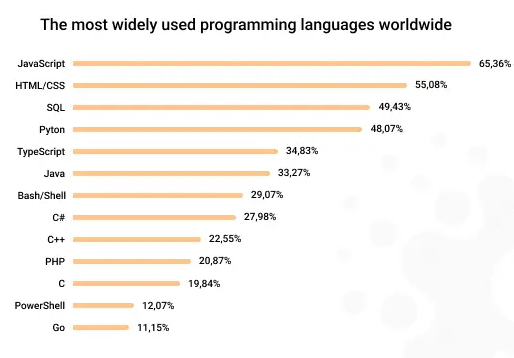
\includegraphics{images/top.png}
	\end{center}
	\fonte{https://www.softermii.com/blog/top-programming-languages-and-frameworks-for-software-development}
\end{figure}
% ----------------------------------------------------------

\subsection{Expo}
O Expo é uma plataforma que simplifica o desenvolvimento de aplicativos móveis usando JavaScript e React Native. Com recursos nativos do dispositivo acessíveis e facilitando a colaboração e distribuição de aplicativos, o Expo oferece uma solução abrangente para criar aplicativos móveis.

Segundo (\textcite{Hugo}) o uso do Expo proporciona uma camada de abstração superior ao React Native, resultando em uma experiência aprimorada no desenvolvimento de software. Com o aumento do 
número de usuários de smartphones, especialmente nas plataformas Android e iOS, a necessidade de criar aplicativos para ambas as plataformas se tornou cada vez mais 
evidente. Nesse contexto, o Expo oferece uma vantagem no desenvolvimento híbrido, simplificando o processo de criação de aplicativos multiplataforma.


\begin{figure}[htb]
	\caption{\label{fig:Fig_1}Expo vantagens}
	\begin{center}
		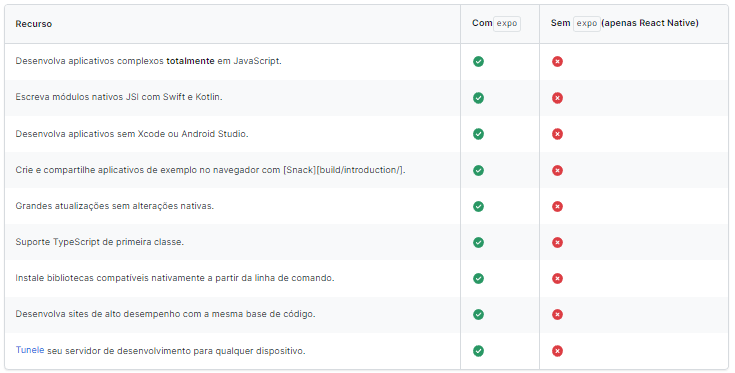
\includegraphics{images/expo.png}
	\end{center}
	\fonte{https://docs.expo.dev/core-concepts/}
\end{figure}

\subsection{Gin}
O framework Gin é uma biblioteca leve e rápida para construção de APIs em Go. Ele se baseia nos princípios do roteamento HTTP e fornece recursos poderosos para o desenvolvimento de aplicativos web escaláveis e de alto desempenho.

Ao utilizar o Gin, os desenvolvedores se beneficiam de uma sintaxe concisa e intuitiva, o que torna a criação de endpoints mais eficiente e produtiva. O framework oferece um roteamento flexível, permitindo mapear os diferentes endpoints para as funções correspondentes de forma clara e organizada.

Além disso, o Gin oferece suporte para a manipulação de parâmetros nas requisições HTTP. Isso permite que os desenvolvedores acessem e processem os dados enviados pelos clientes de forma simples e segura. O framework também oferece recursos para validação de entrada de dados, facilitando a verificação de formatos, tipos e restrições específicas, garantindo a integridade dos dados recebidos.

Outro aspecto importante do Gin é a sua eficiência e desempenho. Ele foi projetado para ser leve e rápido, proporcionando um processamento ágil das requisições. Isso é especialmente relevante em aplicações de grande escala, onde a capacidade de resposta e o tempo de processamento são cruciais.

O framework Gin também oferece recursos avançados, como middleware, que permite adicionar funcionalidades extras às rotas e endpoints da API. Isso inclui autenticação, autorização, logging e muitos outros aspectos que são essenciais para o desenvolvimento de sistemas seguros e escaláveis.

Em resumo, o uso do framework Gin proporciona uma base sólida e eficiente para o desenvolvimento de APIs RESTful. Sua sintaxe concisa, roteamento flexível, manipulação de parâmetros, validação de entrada e recursos avançados garantem a criação de endpoints robustos, escaláveis e de alto desempenho, possibilitando a construção de aplicações web modernas e eficientes.


\subsection{Comparação}
\begin{table}[htb]
    \centering
    \caption{Comparação}
    \label{tab:comparação}
\begin{tabular}{|p{5cm}|p{2cm}|p{2cm}|p{2cm}|}
    \hline
    \textbf{Características} & \textbf{Getninjas} & \textbf{99freelas} & \textbf{Empregai}  \\ \hline
    Diversidade de serviços   & \multicolumn{1}{c|}{\textbf{X}}   & \multicolumn{1}{c|}{\textbf{-}}  & \multicolumn{1}{c|}{\textbf{X}} \\ \hline
	Avaliações e recomendações   & \multicolumn{1}{c|}{\textbf{X}}   & \multicolumn{1}{c|}{\textbf{X}}  & \multicolumn{1}{c|}{\textbf{X}} \\ \hline
    Aplicativo móvel   & \multicolumn{1}{c|}{\textbf{X}}   & \multicolumn{1}{c|}{\textbf{-}}  & \multicolumn{1}{c|}{\textbf{X}} \\ \hline
    Sistema de mensagens   & \multicolumn{1}{c|}{\textbf{?}}   & \multicolumn{1}{c|}{\textbf{X}}  & \multicolumn{1}{c|}{\textbf{?}} \\ \hline
    Possibilidade dos clientes se adicionar   & \multicolumn{1}{c|}{\textbf{-}}   & \multicolumn{1}{c|}{\textbf{-}}  & \multicolumn{1}{c|}{\textbf{X}} \\ \hline
	Avaliação de pessoas conhecidas   & \multicolumn{1}{c|}{\textbf{-}}   & \multicolumn{1}{c|}{\textbf{-}}  & \multicolumn{1}{c|}{\textbf{X}} \\ \hline
	Pagamentos na plataforma   & \multicolumn{1}{c|}{\textbf{-}}   & \multicolumn{1}{c|}{\textbf{X}}  & \multicolumn{1}{c|}{\textbf{?}} \\ \hline
\end{tabular}
    \fonte{Elaborado pelos autores (2023).}
\end{table}
% ---

% ---
% 3 - Capítulo 3
% ---
% ----------------------------------------------------------
\chapter{Desenvolvimento}\label{cap:desenvolvimento}
% ----------------------------------------------------------
Deve-se inserir texto entre as seções.
% ----------------------------------------------------------
\subsection{Lista de requisitos}
Segue os requisitos do projeto
% ----------------------------------------------------------
\begin{quadro}[htb]
	\centering
	\caption{\label{Formatação do texto.}Requisitos funcionais}	
	\begin{tabular}{|l|p{11cm}|}
		\hline
		\textbf{Identificação}    & \textbf{Requisito}\\ \hline
		RF01        			  & Manter usuário\\ \hline
		RF02        			  & Realizar login\\ \hline
		RF03         			  & Cadastro de anúncio\\ \hline
		RF04        			  & Avaliação do profissional\\ \hline
		RF05        			  & Histórico de serviços prestados\\ \hline
		RF06        			  & Avaliação do profissional\\ \hline
	\end{tabular}
	\fonte{\textcite{Elaborado pelos autores(2023)}.}
\end{quadro}

\begin{quadro}[htb]
	\centering
	\caption{\label{Formatação do texto.}Requisitos não funcionais}	
	\begin{tabular}{|l|p{11cm}|}
		\hline
		\textbf{Identificação}    & \textbf{Requisito}\\ \hline
		RNF01        			  & Banco de dados relacional(PostgreSQL)\\ \hline
		RNF02        			  & Interface mobile em ReactJS Native\\ \hline
	\end{tabular}
	\fonte{\textcite{Elaborado pelos autores(2023)}.}
\end{quadro}

\subsection{Descrição dos requisitos funcionais }

\begin{quadro}[htb]
	\centering
	\caption{\label{Formatação do texto.}Descrição RF01}	
	\begin{tabular}{|l|p{11cm}|}
		\hline
		\textbf{Nome}    & Manter usuário\\ \hline
		\textbf{Tipo}    & Funcional\\ \hline
		\multicolumn{2}{|c|}{Descrição}\\ \hline
		\multicolumn{2}{|p{12cm}|}{
			O sistema deve permitir o cadastro de usuários e o gerenciamento de suas informações. \newline
			\newline Critérios de Aceitação: \newline
			O sistema deve permitir o cadastro de novos clientes com as informações básicas (nome, e-mail, senha, CPF, cidade, endereço e telefone); \newline
			\newline O sistema deve permitir o cadastro de novos prestadores com as informações básicas (nome, e-mail, senha, CPF, ou CNPJ, cidade, categoria do serviços prestados e telefone); \newline
			\newline O sistema deve permitir a atualização das informações do usuário, incluindo nome, e-mail e senha; \newline
			\newline O sistema deve permitir a exclusão do usuário; \newline
			O sistema deve garantir a segurança das informações dos usuários, armazenando as senhas de forma criptografada.
			} \\ \hline
	\end{tabular}
	\fonte{\textcite{Elaborado pelos autores(2023)}.}
\end{quadro}

\begin{quadro}[htb]
	\centering
	\caption{\label{Formatação do texto.}Descrição RF02}	
	\begin{tabular}{|l|p{11cm}|}
		\hline
		\textbf{Nome}    & Realizar login\\ \hline
		\textbf{Tipo}    & Funcional\\ \hline
		\multicolumn{2}{|c|}{Descrição}\\ \hline
		\multicolumn{2}{|p{12cm}|}{
			O sistema deve permitir que os usuários realizem login para acessar suas contas. \newline
			\newline Critérios de Aceitação: \newline
			O sistema deve apresentar um formulário de login com os campos de e-mail e senha; \newline
			\newline O sistema deve validar as informações de login e permitir o acesso ao usuário caso as informações estejam corretas;\newline
			\newline O sistema deve apresentar uma mensagem de erro caso as informações de login estejam incorretas;
			} \\ \hline
	\end{tabular}
	\fonte{\textcite{Elaborado pelos autores(2023)}.}
\end{quadro}

\begin{quadro}[htb]
	\centering
	\caption{\label{Formatação do texto.}Descrição RF03}	
	\begin{tabular}{|l|p{11cm}|}
		\hline
		\textbf{Nome}    & Cadastro de anúncio\\ \hline
		\textbf{Tipo}    & Funcional\\ \hline
		\multicolumn{2}{|c|}{Descrição}\\ \hline
		\multicolumn{2}{|p{12cm}|}{
			O sistema deve permitir que os clientes cadastrem seus anúncios de serviços. \newline
			\newline Critérios de Aceitação: \newline
			O sistema deve apresentar um formulário para o cadastro de anúncio, contendo informações como título, descrição, categoria eu localização; \newline
			\newline O sistema deve permitir que o cliente edite e exclua seus anúncios;\newline
			\newline O sistema deve validar as informações inseridas pelo cliente, garantindo que o anúncio contenha informações suficientes e válidas para ser publicado.
			} \\ \hline
	\end{tabular}
	\fonte{\textcite{Elaborado pelos autores(2023)}.}
\end{quadro}

\begin{quadro}[htb]
	\centering
	\caption{\label{Formatação do texto.}Descrição RF04}	
	\begin{tabular}{|l|p{11cm}|}
		\hline
		\textbf{Nome}    & Avaliação do profissional\\ \hline
		\textbf{Tipo}    & Funcional\\ \hline
		\multicolumn{2}{|c|}{Descrição}\\ \hline
		\multicolumn{2}{|p{12cm}|}{
			O sistema deve permitir que os clientes avaliem os prestadores de serviço após a realização do serviço. \newline
			\newline Critérios de Aceitação: \newline
			O sistema deve apresentar um campo de avaliação com uma escala numérica ou de estrelas e um campo para o cliente deixar um comentário sobre a qualidade do serviço prestado; \newline
			\newline O sistema deve permitir que o cliente avalie apenas os prestadores de serviço que já foram contratados por ele; \newline
			\newline O sistema deve disponibilizar as avaliações dos prestadores de serviço para que outros clientes possam consultar antes de contratar os serviços dos mesmos.
			} \\ \hline
	\end{tabular}
	\fonte{\textcite{Elaborado pelos autores(2023)}.}
\end{quadro}

\begin{quadro}[htb]
	\centering
	\caption{\label{Formatação do texto.}Descrição RF05}	
	\begin{tabular}{|l|p{11cm}|}
		\hline
		\textbf{Nome}    & Histórico de serviços prestados\\ \hline
		\textbf{Tipo}    & Funcional\\ \hline
		\multicolumn{2}{|c|}{Descrição}\\ \hline
		\multicolumn{2}{|p{12cm}|}{
			O sistema deve permitir que os prestadores de serviço visualizem seu histórico de serviços prestados. \newline
			\newline Critérios de Aceitação: \newline
			O sistema deve exibir uma lista de todos os serviços prestados pelo prestador, com informações como o título do anúncio e a data de realização; \newline
			\newline O sistema deve permitir que o cliente avalie apenas os prestadores de serviço que já foram contratados por ele; \newline
			\newline O sistema deve disponibilizar as avaliações dos prestadores de serviço para que outros clientes possam consultar antes de contratar os serviços dos mesmos.
			} \\ \hline
	\end{tabular}
	\fonte{\textcite{Elaborado pelos autores(2023)}.}
\end{quadro}

\begin{quadro}[htb]
	\centering
	\caption{\label{Formatação do texto.}Descrição RF06}	
	\begin{tabular}{|l|p{11cm}|}
		\hline
		\textbf{Nome}    & Histórico de serviços prestados\\ \hline
		\textbf{Tipo}    & Funcional\\ \hline
		\multicolumn{2}{|c|}{Descrição}\\ \hline
		\multicolumn{2}{|p{12cm}|}{
			O sistema deve permitir que o cliente tenha acesso ao histórico de serviços contratados por ele, incluindo informações como data, valor, nome do prestador de serviço e avaliação. \newline
			\newline Critérios de Aceitação: \newline
			O sistema deve apresentar uma lista dos serviços contratados pelo cliente;
Cada serviço deve apresentar informações como data, nome do prestador de serviço e avaliação; \newline
			\newline O histórico deve ser atualizado automaticamente após a conclusão do serviço;
			} \\ \hline
	\end{tabular}
	\fonte{\textcite{Elaborado pelos autores(2023)}.}
\end{quadro}

\subsection{Descrição dos requisitos não funcionais }

\begin{quadro}[htb]
	\centering
	\caption{\label{Formatação do texto.}Descrição RNF01}	
	\begin{tabular}{|l|p{11cm}|}
		\hline
		\textbf{Nome}    & Banco de dados relacional(PostgreSQL)\\ \hline
		\textbf{Tipo}    & Não funcional\\ \hline
		\multicolumn{2}{|c|}{Descrição}\\ \hline
		\multicolumn{2}{|p{12cm}|}{
			O sistema deve utilizar um banco de dados relacional PostgreSQL para armazenamento de dados. \newline
			\newline Critérios de Aceitação: \newline
			O banco de dados deve ser implementado em PostgreSQL;
			Deve ser garantida a integridade e consistência dos dados armazenados;\newline
			\newline O esquema do banco de dados deve ser projetado de acordo com as necessidades do sistema; \newline
			\newline O acesso ao banco de dados deve ser realizado através de um usuário com permissões adequadas; \newline
			\newline O sistema deve permitir a exclusão do usuário; \newline
			O banco de dados deve ser capaz de suportar um grande volume de dados e garantir a disponibilidade do sistema.
			} \\ \hline
	\end{tabular}
	\fonte{\textcite{Elaborado pelos autores(2023)}.}
\end{quadro}

\begin{quadro}[htb]
	\centering
	\caption{\label{Formatação do texto.}Descrição RNF02}	
	\begin{tabular}{|l|p{11cm}|}
		\hline
		\textbf{Nome}    & Interface mobile em ReactJS Native utilizando Expo\\ \hline
		\textbf{Tipo}    & Não funcional\\ \hline
		\multicolumn{2}{|c|}{Descrição}\\ \hline
		\multicolumn{2}{|p{12cm}|}{
			O sistema deve utilizar React Native em conjunto com a plataforma Expo para desenvolvimento da interface mobile. \newline
			\newline Critérios de Aceitação: \newline
			A interface deve ser desenvolvida em React Native utilizando a plataforma Expo; \newline
			\newline A interface deve ser responsiva e adaptável a diferentes tamanhos de tela;\newline
			\newline A interface deve ser desenvolvida de acordo com as diretrizes da plataforma para garantir compatibilidade e desempenho.
			} \\ \hline
	\end{tabular}
	\fonte{\textcite{Elaborado pelos autores(2023)}.}
\end{quadro}
% ---

% ---
% 4 - Conclusão
% ---
%\phantompart
% ----------------------------------------------------------
\chapter{PROCESSO DE DESENVOLVIMENTO DE SOFTWARE}\label{cap:desenvolvimento}
% ----------------------------------------------------------
Para \textcite{Pressman2016} os modelos de processos de desenvolvimento 
tradicionais concentram-se em estruturar e ordenar o desenvolvimento de software. As 
atividades e tarefas ocorrem sequencialmente, com diretrizes de progresso bem 
definidas. O autor define algumas atividades genéricas para os processos de 
desenvolvimento de software, sendo elas:
\begin{itemize}[label=$\bullet$]
	\item Comunicação: Levantamento de requisitos.
	\item Planejamento: Estimativas, cronograma, acompanhamento.
	\item Modelagem: Análise, projeto.
	\item Construção: Código, testes.
	\item Entrega/Disponibilização: Entrega, feedback.
	\end{itemize}
	Segundo \textcite{Pressman2016}, o modelo incremental combina os fluxos de processo linear
	e paralelo dos elementos. O modelo incremental aplicasequências lineares de
	forma escalonada, à medida que o tempo vai avançando. Cada sequência linear
	produz incrementos entregáveis do software. \newline
	Segundo \textcite{Pressman2016} destaca que, quando se utiliza um modelo incremental,
	frequentemente o primeiro incremento é um produto essencial. Esse 
	produto essencial é utilizado pelo cliente (ou passa por uma avaliaão detalhada). Como 
	resultado do uso e/ou avaliação, é desenvolvido um planejamento para o incremento
	seguinte. O planejamento já considera a modificação do produto essencial para melhor 
	se adequar às necessidades do cliente e à entrega de recursos e funcionalidades 
	adicionais
	Tendo em vista disso, o seguinte projeto tem como objetivo utilizar o processo 
	incremental para o desenvolvimento do software Empregai, com validações de 
	progresso quinzenais. O código fonte será disponibilizado no GitHub.

% ----------------------------------------------------------
\subsection{Lista de Abreviaturas nos Artefatos do Documento}
Lista de Abreviaturas nos Artefatos do Documento
% ----------------------------------------------------------

% ----------------------------------------------------------
\chapter{REQUISITOS}
% ----------------------------------------------------------
Deve-se inserir texto entre as seções.
% ----------------------------------------------------------
\subsection{Lista de requisitos}
Segue os requisitos do projeto
% ----------------------------------------------------------
\begin{quadro}[htb]
	\centering
	\caption{\label{Formatação do texto.}Requisitos funcionais}	
	\begin{tabular}{|l|p{11cm}|}
		\hline
		\textbf{Identificação}    & \textbf{Requisito}\\ \hline
		RF01        			  & Manter usuário\\ \hline
		RF02        			  & Realizar login\\ \hline
		RF03         			  & Cadastro de anúncio\\ \hline
		RF04        			  & Avaliação do profissional\\ \hline
		RF05        			  & Histórico de serviços prestados\\ \hline
		RF06        			  & Histórico de serviços contratados \\ \hline
		RF07        			  & Candidatar no anúncio \\ \hline
		RF08        			  & Candidatar no anúncio 
		\\ \hline
	\end{tabular}
	\fonte{\textcite{Elaborado pelos autores(2023)}.}
\end{quadro}

\begin{quadro}[htb]
	\centering
	\caption{\label{Formatação do texto.}Requisitos não funcionais}	
	\begin{tabular}{|l|p{11cm}|}
		\hline
		\textbf{Identificação}    & \textbf{Requisito}\\ \hline
		RNF01        			  & Banco de dados relacional(PostgreSQL)\\ \hline
		RNF02        			  & Interface mobile em ReactJS Native\\ \hline
	\end{tabular}
	\fonte{\textcite{Elaborado pelos autores(2023)}.}
\end{quadro}

\subsection{ Lista de Regras de Negócio}

\begin{tabular}{|l|p{8cm}|p{3cm}|}
	\hline
	\textbf{Identificação} & \textbf{Regras de Negócio} & \textbf{Requisito associado} \\ \hline
	RN01 & Validação CPF válido e único. & RF1 \\ \hline
	RN02 & RValidação de email válido e único. & RF02 \\ \hline
	RN03 & O prestador de serviço NÃO poderá se candidatar para, realizar um serviço caso tenha um serviço marcado para a mesma data e hora. & RF07 \\ \hline
	RN04 & O cliente só poderá selecionar um profissional, para realizar o serviço. & RF08 \\ \hline
	RN05 & O cliente só poderá avaliar um profissional após a conclusão do serviço. & RF08, RF04 \\ \hline
	RN06 & O prestador de serviços só poderá ver e se candidatar para serviços relacionados com o seu perfil  & RF07 \\ \hline
	RN07 & O cliente não poderá fazer um anúncio com a data do passado  & RF03 \\ \hline
	RN08 & Caso o anúncio tenha uma data de expiração ele não deverá aparecer em tela e o anunciante deverá ser notificado & RF03 \\ \hline
\end{tabular}


\subsection{Descrição dos requisitos funcionais }

\begin{quadro}[htb]
	\centering
	\caption{\label{Formatação do texto.}Descrição RF01}	
	\begin{tabular}{|l|p{11cm}|}
		\hline
		\textbf{Incremento}    & Iteração 01\\ \hline
		\textbf{Nome}    & Manter usuário\\ \hline
		\textbf{Tipo}    & Funcional\\ \hline
		\multicolumn{2}{|c|}{Descrição}\\ \hline
		\multicolumn{2}{|p{12cm}|}{
			O sistema deve permitir o cadastro de usuários e o gerenciamento de suas informações. \newline
			\newline Critérios de Aceitação: \newline
			O sistema deve permitir o cadastro de novos clientes com as informações básicas (nome, e-mail, senha, CPF, cidade, endereço e telefone); \newline
			\newline O sistema deve permitir o cadastro de novos prestadores com as informações básicas (nome, e-mail, senha, CPF, ou CNPJ, cidade, categoria do serviços prestados e telefone); \newline
			\newline O sistema deve permitir a atualização das informações do usuário, incluindo nome, e-mail e senha; \newline
			\newline O sistema deve permitir a exclusão do usuário; \newline
			O sistema deve garantir a segurança das informações dos usuários, armazenando as senhas de forma criptografada.
			} \\ \hline
	\end{tabular}
	\fonte{\textcite{Elaborado pelos autores(2023)}.}
\end{quadro}

\begin{quadro}[htb]
	\centering
	\caption{\label{Formatação do texto.}Descrição RF02}	
	\begin{tabular}{|l|p{11cm}|}
		\hline
		\textbf{Nome}    & Realizar login\\ \hline
		\textbf{Tipo}    & Funcional\\ \hline
		\multicolumn{2}{|c|}{Descrição}\\ \hline
		\multicolumn{2}{|p{12cm}|}{
			O sistema deve permitir que os usuários realizem login para acessar suas contas. \newline
			\newline Critérios de Aceitação: \newline
			O sistema deve apresentar um formulário de login com os campos de e-mail e senha; \newline
			\newline O sistema deve validar as informações de login e permitir o acesso ao usuário caso as informações estejam corretas;\newline
			\newline O sistema deve apresentar uma mensagem de erro caso as informações de login estejam incorretas;
			} \\ \hline
		\multicolumn{1}{|l|}{Descrição} {
			asassad
		}
	\end{tabular}
	\fonte{\textcite{Elaborado pelos autores(2023)}.}
\end{quadro}

\begin{quadro}[htb]
	\centering
	\caption{\label{Formatação do texto.}Descrição RF03}	
	\begin{tabular}{|l|p{11cm}|}
		\hline
		\textbf{Nome}    & Cadastro de anúncio\\ \hline
		\textbf{Tipo}    & Funcional\\ \hline
		\multicolumn{2}{|c|}{Descrição}\\ \hline
		\multicolumn{2}{|p{12cm}|}{
			O sistema deve permitir que os clientes cadastrem seus anúncios de serviços. \newline
			\newline Critérios de Aceitação: \newline
			O sistema deve apresentar um formulário para o cadastro de anúncio, contendo informações como título, descrição, categoria eu localização; \newline
			\newline O sistema deve permitir que o cliente edite e exclua seus anúncios;\newline
			\newline O sistema deve validar as informações inseridas pelo cliente, garantindo que o anúncio contenha informações suficientes e válidas para ser publicado.
			} \\ \hline
	\end{tabular}
	\fonte{\textcite{Elaborado pelos autores(2023)}.}
\end{quadro}

\begin{quadro}[htb]
	\centering
	\caption{\label{Formatação do texto.}Descrição RF04}	
	\begin{tabular}{|l|p{11cm}|}
		\hline
		\textbf{Nome}    & Avaliação do profissional\\ \hline
		\textbf{Tipo}    & Funcional\\ \hline
		\multicolumn{2}{|c|}{Descrição}\\ \hline
		\multicolumn{2}{|p{12cm}|}{
			O sistema deve permitir que os clientes avaliem os prestadores de serviço após a realização do serviço. \newline
			\newline Critérios de Aceitação: \newline
			O sistema deve apresentar um campo de avaliação com uma escala numérica ou de estrelas e um campo para o cliente deixar um comentário sobre a qualidade do serviço prestado; \newline
			\newline O sistema deve permitir que o cliente avalie apenas os prestadores de serviço que já foram contratados por ele; \newline
			\newline O sistema deve disponibilizar as avaliações dos prestadores de serviço para que outros clientes possam consultar antes de contratar os serviços dos mesmos.
			} \\ \hline
	\end{tabular}
	\fonte{\textcite{Elaborado pelos autores(2023)}.}
\end{quadro}

\begin{quadro}[htb]
	\centering
	\caption{\label{Formatação do texto.}Descrição RF05}	
	\begin{tabular}{|l|p{11cm}|}
		\hline
		\textbf{Nome}    & Histórico de serviços prestados\\ \hline
		\textbf{Tipo}    & Funcional\\ \hline
		\multicolumn{2}{|c|}{Descrição}\\ \hline
		\multicolumn{2}{|p{12cm}|}{
			O sistema deve permitir que os prestadores de serviço visualizem seu histórico de serviços prestados. \newline
			\newline Critérios de Aceitação: \newline
			O sistema deve exibir uma lista de todos os serviços prestados pelo prestador, com informações como o título do anúncio e a data de realização; \newline
			\newline O sistema deve permitir que o cliente avalie apenas os prestadores de serviço que já foram contratados por ele; \newline
			\newline O sistema deve disponibilizar as avaliações dos prestadores de serviço para que outros clientes possam consultar antes de contratar os serviços dos mesmos.
			} \\ \hline
	\end{tabular}
	\fonte{\textcite{Elaborado pelos autores(2023)}.}
\end{quadro}

\begin{quadro}[htb]
	\centering
	\caption{\label{Formatação do texto.}Descrição RF06}	
	\begin{tabular}{|l|p{11cm}|}
		\hline
		\textbf{Nome}    & Histórico de serviços contratados\\ \hline
		\textbf{Tipo}    & Funcional\\ \hline
		\multicolumn{2}{|c|}{Descrição}\\ \hline
		\multicolumn{2}{|p{12cm}|}{
			O sistema deve permitir que o cliente tenha acesso ao histórico de serviços contratados por ele, incluindo informações como data, valor, nome do prestador de serviço e avaliação. \newline
			\newline Critérios de Aceitação: \newline
			O sistema deve apresentar uma lista dos serviços contratados pelo cliente; \newline
            Cada serviço deve apresentar informações como data, nome do prestador de serviço e avaliação; \newline
			\newline O histórico deve ser atualizado automaticamente após a conclusão do serviço;
			} \\ \hline
	\end{tabular}
	\fonte{\textcite{Elaborado pelos autores(2023)}.}
\end{quadro}

\begin{quadro}[htb]
	\centering
	\caption{\label{Formatação do texto.}Descrição RF07}	
	\begin{tabular}{|l|p{11cm}|}
		\hline
		\textbf{Nome}    & Candidatar no anúncio\\ \hline
		\textbf{Tipo}    & Funcional\\ \hline
		\multicolumn{2}{|c|}{Descrição}\\ \hline
		\multicolumn{2}{|p{12cm}|}{
			O sistema deve permitir que prestadores de serviços possam se candidatar a anúncios criados pelos clientes. \newline
			\newline Critérios de Aceitação: \newline
			O prestador de serviços deve ser capaz de visualizar os anúncios disponíveis para candidatura; \newline
            O prestador de serviços deve poder se candidatar a um anúncio ao clicar em um botão específico; \newline
			O cliente deve ser notificado da candidatura do prestador de serviços; \newline
			O cliente deve ser capaz de visualizar as candidaturas recebidas para seu anúncio; \newline
			O cliente deve ser capaz de selecionar e contatar o prestador de serviços escolhido para o anúncio.
			} \\ \hline
	\end{tabular}
	\fonte{\textcite{Elaborado pelos autores(2023)}.}
\end{quadro}

\begin{quadro}[htb]
	\centering
	\caption{\label{Formatação do texto.}Descrição RF08}	
	\begin{tabular}{|l|p{11cm}|}
		\hline
		\textbf{Nome}    & Concluir o anúncio\\ \hline
		\textbf{Tipo}    & Funcional\\ \hline
		\multicolumn{2}{|c|}{Descrição}\\ \hline
		\multicolumn{2}{|p{12cm}|}{
			O sistema deve permitir que clientes concluam um anúncio após a seleção de um prestador de serviços. \newline
			\newline Critérios de Aceitação: \newline
			O cliente deve ser capaz de visualizar a lista de candidaturas recebidas para o anúncio; \newline
            O cliente deve ser capaz de selecionar um prestador de serviços para realizar o trabalho; \newline
			O cliente deve ser capaz de confirmar a seleção do prestador de serviços; \newline
			O prestador de serviço de se informado que sua candidatura foi aceita; \newline
			O sistema deve permitir que o cliente avalie o prestador de serviços após a conclusão do trabalho.
			} \\ \hline
	\end{tabular}
	\fonte{\textcite{Elaborado pelos autores(2023)}.}
\end{quadro}

\subsection{Descrição dos requisitos não funcionais }

\begin{quadro}[htb]
	\centering
	\caption{\label{Formatação do texto.}Descrição RNF01}	
	\begin{tabular}{|l|p{11cm}|}
		\hline
		\textbf{Nome}    & Banco de dados relacional(PostgreSQL)\\ \hline
		\textbf{Tipo}    & Não funcional\\ \hline
		\multicolumn{2}{|c|}{Descrição}\\ \hline
		\multicolumn{2}{|p{12cm}|}{
			O sistema deve utilizar um banco de dados relacional PostgreSQL para armazenamento de dados. \newline
			\newline Critérios de Aceitação: \newline
			O banco de dados deve ser implementado em PostgreSQL;
			Deve ser garantida a integridade e consistência dos dados armazenados;\newline
			\newline O esquema do banco de dados deve ser projetado de acordo com as necessidades do sistema; \newline
			\newline O acesso ao banco de dados deve ser realizado através de um usuário com permissões adequadas; \newline
			\newline O sistema deve permitir a exclusão do usuário; \newline
			O banco de dados deve ser capaz de suportar um grande volume de dados e garantir a disponibilidade do sistema.
			} \\ \hline
	\end{tabular}
	\fonte{\textcite{Elaborado pelos autores(2023)}.}
\end{quadro}

\begin{quadro}[htb]
	\centering
	\caption{\label{Formatação do texto.}Descrição RNF02}	
	\begin{tabular}{|l|p{11cm}|}
		\hline
		\textbf{Nome}    & Interface mobile em ReactJS Native utilizando Expo\\ \hline
		\textbf{Tipo}    & Não funcional\\ \hline
		\multicolumn{2}{|c|}{Descrição}\\ \hline
		\multicolumn{2}{|p{12cm}|}{
			O sistema deve utilizar React Native em conjunto com a plataforma Expo para desenvolvimento da interface mobile. \newline
			\newline Critérios de Aceitação: \newline
			A interface deve ser desenvolvida em React Native utilizando a plataforma Expo; \newline
			\newline A interface deve ser responsiva e adaptável a diferentes tamanhos de tela;\newline
			\newline A interface deve ser desenvolvida de acordo com as diretrizes da plataforma para garantir compatibilidade e desempenho.
			} \\ \hline
	\end{tabular}
	\fonte{\textcite{Elaborado pelos autores(2023)}.}
\end{quadro}
% ---

% ----------------------------------------------------------
% ELEMENTOS PÓS-TEXTUAIS
% ----------------------------------------------------------
\postextual
% ----------------------------------------------------------

% ----------------------------------------------------------
% Referências bibliográficas
% ----------------------------------------------------------
\begingroup
    \SingleSpacing\printbibliography[title=REFERÊNCIAS]
\endgroup

% ----------------------------------------------------------
% Glossário
% ----------------------------------------------------------
%
% Consulte o manual da classe abntex2 para orientações sobre o glossário.
%
%\glossary

% ----------------------------------------------------------
% Apêndices
% ----------------------------------------------------------

% ---
% Inicia os apêndices
% ---
\begin{apendicesenv}
%	\partapendices* 
	% % ----------------------------------------------------------
% \chapter{Descrição}
% % ----------------------------------------------------------

% Textos elaborados pelo autor, a fim de completar a sua argumentação. Deve ser precedido da palavra APÊNDICE, identificada por letras maiúsculas consecutivas, travessão e pelo respectivo título. Utilizam-se letras maiúsculas dobradas quando esgotadas as letras do alfabeto. 

% \begin{quadro}[htb]
% 	\centering
% 	\caption{\label{qua:Quadro_2}Modelo A.}	
% \begin{tabular}{|l|l|}
% \hline
% xxxx              & yyyyyyyyyyyyyyy    \\
% \hline
% xxxx              & yyyyyyyyyyyyyyy    \\
% \hline
% xxxx              & yyyyyyyyyyyyyyy    \\
% \hline
% xxxx              & yyyyyyyyyyyyyyy    \\
% \hline
% xxxx              & yyyyyyyyyyyyyyy    \\
% \hline
% xxxx              & yyyyyyyyyyyyyyy    \\
% \hline
% xxxx              & yyyyyyyyyyyyyyy    \\
% \hline
% rrrrrrrrrrrrrrrrr & eeeeeeeeeeeeeeeee  \\
% \hline
% xxxx              & yyyyyyyyyyyyyyy    \\
% \hline
% xxxx              & yyyyyyyyyyyyyyy    \\
% \hline
% rrrrrrrrrrrrrrrrr & eeeeeeeeeeeeeeeee  \\
% \hline
% xxxx              & yyyyyyyyyyyyyyy    \\
% \hline
%                   & ttttttttttttttttt  \\
% \hline
% rrrrrrrrrrrrrrrrr & eeeeeeeeeeeeeeeee  \\
% \hline
% ttttttttttttt     &                    \\
% \hline
% rrrrrrrrrrrrrrrrr & eeeeeeeeeeeeeeeee  \\
% \hline
% rrrrrrrrrrrrrrrrr & eeeeeeeeeeeeeeeee  \\
% \hline
%                   & gggggggggggggggggg \\
% \hline
% rrrrrrrrrrrrrrrrr & eeeeeeeeeeeeeeeee  \\
% \hline
% rrrrrrrrrrrrrrrrr & eeeeeeeeeeeeeeeee  \\
% \hline
% rrrrrrrrrrrrrrrrr & eeeeeeeeeeeeeeeee  \\
% \hline
% rrrrrrrrrrrrrrrrr & eeeeeeeeeeeeeeeee  \\
% \hline
% \end{tabular}
% \fonte{Elaborada pelo autor (2016).}
% \end{quadro}
\end{apendicesenv}
% ---


% ----------------------------------------------------------
% Anexos
% ----------------------------------------------------------

% ---
% Inicia os anexos
% ---
\begin{anexosenv}
%	\partanexos*
	% % ----------------------------------------------------------
% \chapter{Descrição}
% % ----------------------------------------------------------

% São documentos não elaborados pelo autor que servem como fundamentação (mapas, leis, estatutos). Deve ser precedido da palavra ANEXO, identificada por letras maiúsculas consecutivas, travessão e pelo respectivo título. Utilizam-se letras maiúsculas dobradas quando esgotadas as letras do alfabeto. 

\end{anexosenv}

%---------------------------------------------------------------------
% INDICE REMISSIVO
%---------------------------------------------------------------------
%\phantompart
%\printindex
%---------------------------------------------------------------------

\end{document}
